%! Author = luciano
%! Date = 22/01/2020

% Preamble
\documentclass[11pt]{article}

% Packages
\usepackage{amsmath}
\usepackage[gobble=auto,
rerun=always
]{pythontex}
\usepackage{fancyvrb}
\usepackage{python}
\usepackage{csquotes}
\usepackage{cleveref}
\usepackage{enumerate}
\usepackage[utf8]{inputenc}
\usepackage[english]{babel}

\usepackage[ruled,linesnumbered,lined,boxed,commentsnumbered]{algorithm2e}
\SetStartEndCondition{ }{}{}%
\SetKwProg{Fn}{def}{\string:}{}
\SetKwInOut{Input}{Input}\SetKwInOut{Output}{Output}
\SetKwFunction{Range}{range}%%
\SetKwFunction{Len}{len}%%
\SetKwFunction{Statistic}{stat\_function}
\SetKwFunction{FnBoots}{bootstrap}
\SetKwFunction{FnBootsNP}{bootstrap\_np}
\SetKwArray{Data}{data}
\SetKwArray{Samples}{array\_of\_samples}
\SetKwArray{Sample}{sample$_{b}$}
\SetKwArray{Results}{result\_array}
\SetKwProg{MP}{Parallel:}{:}{end}
\SetKw{KwTo}{in}\SetKwFor{For}{for}{\string:}{} \SetKwIF{If}{ElseIf}{Else}{if}{:}{elif}{else:}{} \SetKwFor{While}{while}{:}{fintq}
\newcommand{\forcond}{$b=0$ \KwTo $B$}
\renewcommand{\forcond}{$b$ \KwTo\Range{$B$}} \AlgoDontDisplayBlockMarkers\SetAlgoNoEnd\SetAlgoNoLine%

\usepackage[
backend=biber,
style=authoryear
]{biblatex}
\usepackage{graphicx}
\usepackage{float}

\addbibresource{References.bib}

% Document
\begin{document}

\begin{titlepage}

\newcommand{\HRule}{\rule{\linewidth}{0.5mm}} % Defines a new command for the horizontal lines, change thickness here

\center % Center everything on the page

%----------------------------------------------------------------------------------------
%	HEADING SECTIONS
%----------------------------------------------------------------------------------------

\textsc{\LARGE London School of Economics and Political Science}\\[1.0cm] % Name of your university/college
\textsc{\Large ST444 Statistical Computing}\\[0.5cm] % Major heading such as course name
\textsc{\large Project I}\\[0.5cm] % Minor heading such as course title

%----------------------------------------------------------------------------------------
%	TITLE SECTION
%----------------------------------------------------------------------------------------

\HRule \\[0.4cm]
{ \Large \bfseries Bootstrapping Algorithm: Parallel Computing Implementation and Analysis}\\[0.4cm] % Title of your document
\HRule \\[1.5cm]

%----------------------------------------------------------------------------------------
%	AUTHOR SECTION
%----------------------------------------------------------------------------------------

\begin{minipage}{0.4\textwidth}
\begin{flushleft} \large
\emph{Authors (Group 4):}\\
Frayling \textsc{Lora} \\ % Your name
X \textsc{Li} \\
Perfetti \textsc{Luciano} \\
Pizzutti \textsc{Jonathan} \\
\end{flushleft}
\end{minipage}
~
\begin{minipage}{0.4\textwidth}
\begin{flushright} \large
\emph{Professor:} \\
Dr. Yining \textsc{Chen} % Supervisor's Name
\end{flushright}
\end{minipage}\\[2cm]

%----------------------------------------------------------------------------------------
%	DATE SECTION
%----------------------------------------------------------------------------------------

{\large \today}\\[2cm] % Date, change the \today to a set date if you want to be precise

%----------------------------------------------------------------------------------------
%	LOGO SECTION
%----------------------------------------------------------------------------------------


\includegraphics{lse-logo.jpg}\\[1cm] % Include a department/university logo - this will require the graphicx package

%----------------------------------------------------------------------------------------

\vfill % Fill the rest of the page with whitespace

\end{titlepage}

\newpage

\tableofcontents

\section{Introduction}\label{sec:Introduction}

As computing power has dramatically increased in recent decades, the use of bootstrapping as a fundamental data analysis
tool has also surged.(\cite{Boos}) Bootstrapping is a general statistical technique for estimating unknown quantities utilizing random
resampling with replacement for sample data.(\cite{Boos}) This method is often used to approximate standard errors, confidence intervals,
and probability values for test statistics for a given distribution of data.(\cite{Boos}) The term "bootstrapping" was coined by Bradley
Efron in 1979 as a reference to the adage of "pulling oneself up by one's own bootstraps" since the technique approximates
statistical figures utilizing the sample data themselves instead of any external assumptions.(\cite{gunter_1994})

\medskip

The key approach behind bootstrapping is the random sampling of a given number of values from sample data with replacement.(\cite{efron1982jackknife})
Sampling with replacement means that selected values are not removed from the distribution, which allows certain values to be
selected multiple times while other values may not be selected at all.(\cite{efron1982jackknife}) This process maintains the data structure while
reshuffling the values to calculate sample statistics and ultimately estimate the population statistics.(\cite{efron1982jackknife}) Since biases
can be present in this process, statisticians have attempted to provide more accurate results with procedural variants,
including parametric bootstrapping, nonparametric bootstrapping, and Bayesian bootstrapping.(\cite{efron2003})

\medskip

Although the resampling of sample data may not intuitively seem to provide new insights, bootstrapping works by avoiding
assumptions about the population distribution and utilizing the only information available, the sample data, to create a
distribution that may closely resemble that of the population.(\cite{efron2003}) Further theoretical justifications for bootstrapping have
been described in by Peter Hall in "On Bootstrap Confidence Intervals in Nonparametic Regression" (1992),
Dimitris N. Politis, Joseph P. Romano, and Michael Wolf in "Subsampling" (1999) , and S. N. Lahiri in "Resampling Methods for Dependent Data" (2003).

\medskip

Bootstrapping has several methodological advantages. The process enables statistical inferences to be drawn from small
samples when additional information is not available, which is often the case due to the time and cost of gathering more
data.(\cite{Singh_bootstrap}) The approach also does not make assumptions about the data distributions and can consequently be helpful with
non-normal distributions.(\cite{Singh_bootstrap}) Moreover, the simplicity of the bootstrapping calculation is useful when dealing with complex
distributions, distributions that have unknown properties, or problems without an established statistical calculation.(\cite{Singh_bootstrap})
These advantages lead bootstrapping to be more accurate than other prominent methodologies, including the Jackknife, in
many circumstances.(\cite{diciccio1996})

\medskip

However, bootstrapping is also faced with multiple drawbacks. The methodology is generally not effective in estimating
population minimums or maximums, determining the sample mean when the population variance is infinite, and identifying
the sample median if there is population density discontinuity at the population median.(\cite{Singh_bootstrap}) Similarly, bootstrapping does
not work well with sample eigenvalues in cases where population eigenvalues have multiplicity. Another disadvantage of
the technique is the necessity for a large quantity of sampling simulations that require high levels of computation,
especially compared to similar approaches such as the Jackknife.(\cite{diciccio1996})

\medskip

Although computational intensity hindered the spread of bootstrapping at its inception, subsequent technological and
computational developments have created new opportunities to execute such demanding calculations.(\cite{Boos}) An especially
impactful development is parallel computing, which allows computational functions to be carried out simultaneously to
process high amounts of information in shorter periods of time.(\cite{Kindervater}) The technique often involves breaking large calculations
into smaller ones and utilizing multiple processors to execute different functions and reduce computation time.(\cite{Kindervater}) Given the
benefits of this approach, this paper examines how parallel computing can be applied to perform bootstrapping computations in
an efficient and effective manner.


\section{Bootstrapping Functions}\label{sec:bootstrapping-functions}

\subsection{Basic Algorithm}\label{subsec:basic-algorithm}

Before explaining the Bootstrapping algorithm, we should first define the different steps need to accomplish this process.
According to \cite{LW04} we can define $T_n = g(X_1, \dots, X_n)$ as an statistic that depends on the data, and we can then apply
bootstrapping as a procedure to estimate the standard error and confidence intervals of $T_n$ for statistical inference.
To explain the bootstrap theory, \cite{LW04} first proves that by using the law of large numbers, and assuming that we draw an IID sample of $Y_1, \dots, Y_B$,
we can conclude that as $B \rightarrow \infty$

\begin{align}
    \bar{Y} \overset{p}{\to} E(Y)
\end{align}
\begin{align}
    \frac{1}{B} \sum_{j=1}^{B}{(Y_j - \bar{Y})^{2}} \overset{p}{\to} V(Y)
\end{align}

With this result, we can use the sample mean and the sample variance as an approximation for the population mean and variance.
Following the procedures stated by \cite{LW04}, we assume that the data obtained initially follows an empirical distribution
$\hat{F}_n$, from where we can take samples $X_{1}^{*}, \dots, X_{n}^{*}$ and compute $T_{n}^{*} = g(X_{1}^{*}, \dots, X_{n}^{*})$
$B$ times. From this step we will get a vector of $T_{n,1}^{*}, \dots, T_{n,B}^{*}$, from where we can compute the variance
(\cite{LW04}):

\begin{align}
v_{boot} = \frac{1}{B}\sum_{b=1}^{B}{\left( T_{n,b}^{*} - \frac{1}{B} \sum_{r=1}^{B}{T_{n,r}^{*}} \right)^2}
\end{align}

The standard error of the statistic $T_n$ is the square root of the variance, $SE = \sqrt{v_{boot}}$. Although there are
several methods to estimate the confidence interval of the statistics, we are going to use the percentiles of the statistic's
distribution. Consequently, the interval is defined as $C_n = \left(T_{\alpha/2}^{*},T_{1 - \alpha/2}^{*}\right)$.

\medskip

The previous process can be resumed in the Algorithm \ref{alg:AB} to show the steps followed more generally. One can observe that it divides the process
into three main parts: the first part generates $B$ samples, of $n_b$ size, from the original data using replacement,
the second part estimates the statistic $T_{n}$ for each $b$ sample, and, finally, the algorithm estimates the standard error and the
confidence interval. The sampling phase is a loop of size $B$ that applies a sampling function\footnotemark, therefore we can assume that
the time complexity of this process should be linear: $O(n)$, where $n$ is equal to $B$. (Analysis based on \cite{AL09})
Similarly, the second phase, is a process that estimates the statistic for each sample $b$, which should be bounded by
the same time complexity as the first phase if the statistic is simple enough, $O(n)$.
Finally, the last step estimates the variance and the confidence interval, which, assuming as given steps without
their own time complexity, have a constant time complexity $O(1)$, although \cite{GiveHoet12} mentions that this process
could have a time complexity of $O(n^{\frac{1}{2}})$. Under these assumptions, we can expect
for the algorithm to have a linear time complexity $O(n)$, where the slope is determined by the number of samples taken from the
original data and the improvements made by using tools like parallel computing or optimized functions.

\footnotetext{We are assuming that the sampling function has a linear time complexity, since it can be understood as a
loop that generates a random number, under some specific conditions, to select an index of the input. Nonetheless, depending
on the algorithm used, the time complexity can be described by higher levels.}

\medskip

\begin{algorithm}[H]
    \KwData{A sample of a random variable $X$}
    \KwResult{A standard error and confidence interval}
    \tcc{Sampling phase}
    \For{\forcond}{
        select $X_{1, b}^{*}, \dots, X_{n,b}^{*}$ elements of the original data using replacement\; }
    \tcc{Estimation phase}
    \For{\forcond}{
        estimate $T_{n,b}^{*}$ for the $b$-th sample\;}
    \tcc{Results phase}
    estimate the square root of the variance of the statistics and the confidence interval
\caption{Bootstrapping}\label{alg:AB}
\end{algorithm}

\medskip
\medskip

This algorithm could be translated into the following Python code following the steps mentioned by \cite{LW04}. As an
example, we are going to assume that the original data comes from a normal distribution with $\mu = 5$ and $\sigma^2 = 1$
and we want to estimate the standard error and the confidence interval for the statistic, which in this case is the mean.


\begin{pyblock}
import numpy as np
from scipy.stats import norm
# Assume we have a random sample from a normal distribution
np.random.seed(11)
sample_normal = np.random.normal(5, 1, 10000)

# 1. Generate 1000 random samples with replacement
samples = np.array([np.random.choice(sample_normal,
                    size=100, replace=True) for _ in range(1000)])

# 2. Estimate the mean (statistic) for each random sample
mean_dist = np.array([np.mean(x) for x in samples])

# 3. Estimate the standard error and the confidence interval
se_mean = np.sqrt(np.var(mean_dist))
confint_mean = np.percentile(mean_dist, [2.5, 97.5])
print("Standard Error: ",  round(se_mean, 3),
        "\n95% Confidence Interval: ", round(confint_mean[0], 3),
        " - ", round(confint_mean[1], 3))
\end{pyblock}

\printpythontex[verbatim]

\medskip

The main results from the algorithm are the distributions of the statistic obtained from the process, but this product is normally used to estimate the
standard error and the confidence interval of the statistic (i.e. mean).
We can observe the behavior of the bootstrap results in a histogram which, in the case of estimating the mean, illustrates the central
limit theorem. Figure \ref{fig:BootsExample} shows the histogram of the bootstrap samples for the mean with the density kernel of
the observed data (blue line), and the normal distribution (black line). Theory tells us that (\cite{LW04}), by the central limit theorem,
the distribution of the sample mean converges in distribution to a $N(\mu, \sigma^2)$. With this, one can establish
probability statements about the mean of the random variable $X$.


\begin{pycode}
from pylab import *
rc('font', family='serif')
rc('font', size=10.0)
rc('legend', fontsize=10.0)
rc('font', weight='normal')
import numpy as np
from scipy.stats import norm
import seaborn as sns
# Assume we have a random sample from a normal distribution
np.random.seed(11)
sample_normal = np.random.normal(5, 1, 10000)
# 1. Generate 1000 random samples with replacement
samples = np.array([np.random.choice(sample_normal,
                    size=100, replace=True) for _ in range(1000)])
# 2. Estimate the mean (statistic) for each random sample
mean_dist = np.array([np.mean(x) for x in samples])
# 3. Estimate the standard error and the confidence interval
se_mean = np.sqrt(np.var(mean_dist))
confint_mean = np.percentile(mean_dist, [2.5, 97.5])
figure(figsize=(4, 2.5))
axvspan(confint_mean[0], confint_mean[1], facecolor='g', alpha=0.4, ymin=0, ymax=0.05)
sns.distplot(mean_dist, axlabel='Histogram of Bootstrap Samples', fit = norm)
axvline(x = 5, linewidth=2, color='r', alpha = 0.5)
axvline(x=5 - se_mean, linewidth=2, color='orange', ymin=0, ymax=0.1, alpha = 0.8)
axvline(x=5 + se_mean, linewidth=2, color='orange', ymin=0, ymax=0.1, alpha = 0.8)
xlabel('Statistic values')
ylabel('Frequency')
savefig('mean_dist.pdf', transparent=True)
\end{pycode}

\begin{figure}[H]
    \begin{center}
        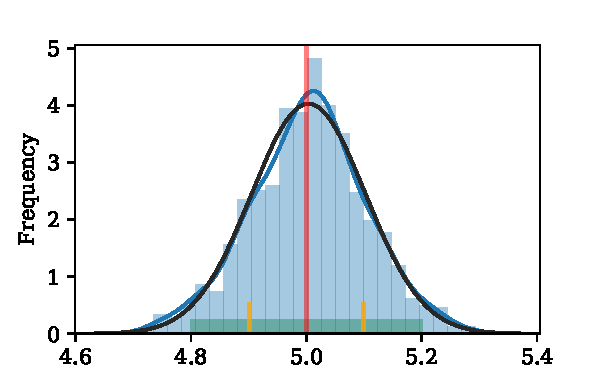
\includegraphics{mean_dist.pdf}
    \end{center}
    \caption{Histogram and density plot of the bootstrap samples. \textit{Note}:
    confidence interval in green area, standard errors in orange and normal distribution in black}\label{fig:BootsExample}
\end{figure}

\medskip

The algorithm implemented shows the expected results with respect to the statistical objectives, however, the main focus
of this study is to analyze the performance of bootstrapping when using parallel computing. Therefore, we are going to ignore
the last phase of the algorithm and concentrate on the first two. The next sections will divide
the problem between a non-parallel version (i.e.\ serial) and a parallel implementation of the bootstrapping algorithm.

\subsection{Serial Algorithms}\label{subsec:serial-algorithms}

The serial version of bootstrapping replicates the steps followed by the Algorithm \ref{alg:AB} with only one processor
of the computer. At this point, to construct a function that executes the algorithm we have to consider the generation
of random numbers for the sampling phase as a main aspect. We decided to use two types of generators to understand how the performance of
the algorithm can change based on specific changes on each step. The two options are: the \texttt{random} package
of python core libraries (Algorithm \ref{alg:AB2}) and \texttt{Numpy} package (Algorithm \ref{alg:AB3}). It is noteworthy
that the first implementation uses a nested loop (line \ref{NestedLoop}), multiplying the linear time complexity by a constant
form $O(mn)$, where $m$ is the size of the samples.\footnotemark Therefore, we can expect that the time complexity of the function
that uses \texttt{numpy} is bounded by the function without \texttt{numpy}.

\footnotetext{Although if the $m = n$, then we will have a $O(n^2)$ time complexity}

\medskip

\begin{algorithm}[H]
    \Input{A sample of a random variable $X$}
    \Output{A object with the standard error and confidence interval}
    \BlankLine
    \Fn{\FnBoots{input, statistic function, number of samples, size of sample}}{
    \tcc{Sampling phase}
    \For{\forcond}{\label{ForSerial1}
        \For{$j$ \KwTo \Range{size of samples}}{\label{NestedLoop}
        \tcp{Using \texttt{random.randint} module}
        \textit{index} = create a random integer $\in$ [0, \Len{\Data{n}} - 1]\;
        \Sample{$j$} = \Data{\textit{index}}\;}
    }

    \tcc{Estimation phase}
    \For{\forcond}{
        \Results{b} = \Statistic{\Samples{b}}\;}
    \tcc{Results phase}
    estimate the square root of the variance of the statistics and the confidence interval\;
    }
\caption{Serial Bootstrapping without \texttt{Numpy}}\label{alg:AB2}
\end{algorithm}

\medskip

On the other hand, on Algorithm \ref{alg:AB3} we replicated the Algorithm \ref{alg:AB2} using the \texttt{numpy} package
to generate the samples from the original data.
Since \texttt{numpy} is a scientific package made to optimize processes like bootstrapping, we
expect a improvement in terms of performance when both functions are compared. The Algorithm \ref{alg:AB3} enumerates the
steps taken by the function to execute the bootstrapping. The main difference with the previous function resides in the
\texttt{for loop} at line \ref{ForSerialNP1} in Algorithm \ref{alg:AB3}, since we avoided the introduction of an additional
\texttt{for loop}. Therefore, we could assume that the time complexity of this algorithm is $O(n)$, since it just performs
the sample and estimation in one \texttt{for loop}.

\begin{algorithm}[H]
    \Input{A sample of a random variable $X$}
    \Output{A object with the standard error and confidence interval}
    \BlankLine
    \Fn{\FnBootsNP{input, statistic function, number of samples, size of sample}}{
    \tcc{Sampling phase and Estimation phase}
    \For{\forcond}{\label{ForSerialNP1}
        \tcp{Using \texttt{numpy.random.choice}}
        \Samples{b} = create a random sample of determined size from \Data \;
        \Results{b} = \Statistic{\Samples{b}}\;}

    \tcc{Results phase}
    estimate the square root of the variance of the statistics and the confidence interval\;
    }
\caption{Serial Bootstrapping with \texttt{Numpy}}\label{alg:AB3}
\end{algorithm}

\medskip

To further analyze the performance of the algorithms, we first implemented a test to generate a range of $B$ samples, since
this is the argument of the bootstrap function that could affect the performance of the functions. The range of the test
has a minimum of $B = 1,000$ samples up to $B = 1,000,000$ samples by steps of $10,000$. For each implementation of the
algorithm we time the performance using the \texttt{timeit} module of Python libraries, which returns an average time for
each run. The results are presented in the Figure \ref{fig:SerialTest}, where the straight blue line is the function
without \texttt{numpy}, and the dashed line is the function in Algorithm \ref{alg:AB3}. In average, the function with Numpy
is 8.64 times faster than the function without this package, confirming our hypothesis on the difference of the time complexity
between both algorithms.

\medskip

\begin{pycode}
from pylab import *
rc('font', family='serif')
rc('font', size=8.0)
rc('legend', fontsize=8.0)
rc('font', weight='normal')
import numpy as np
import pandas as pd
import matplotlib.ticker as ticker
from scipy.stats import norm
import seaborn as sns
data = pd.read_pickle('data/NoNPvsNPv2.pkl')
data_wo = data.loc[:, ['Serial', 'SerialNP']]
data_wo = data_wo.rename(columns={"Serial": "Without Numpy", "SerialNP": "With Numpy"})
clf()
figure(figsize=(5, 4.5))
sns.set(style='darkgrid', palette='Paired')
p = sns.lineplot(data=data_wo, dashes=[(None, None), (2, 2)])
p.xaxis.set_major_formatter(ticker.FuncFormatter(lambda x, pos: '{:,.0f}'.format(x)))
p.set(xlabel = 'Size (number of samples)', ylabel = 'Running Time')
savefig('serial_test.pdf')
\end{pycode}

\begin{figure}[H]
    \begin{center}
        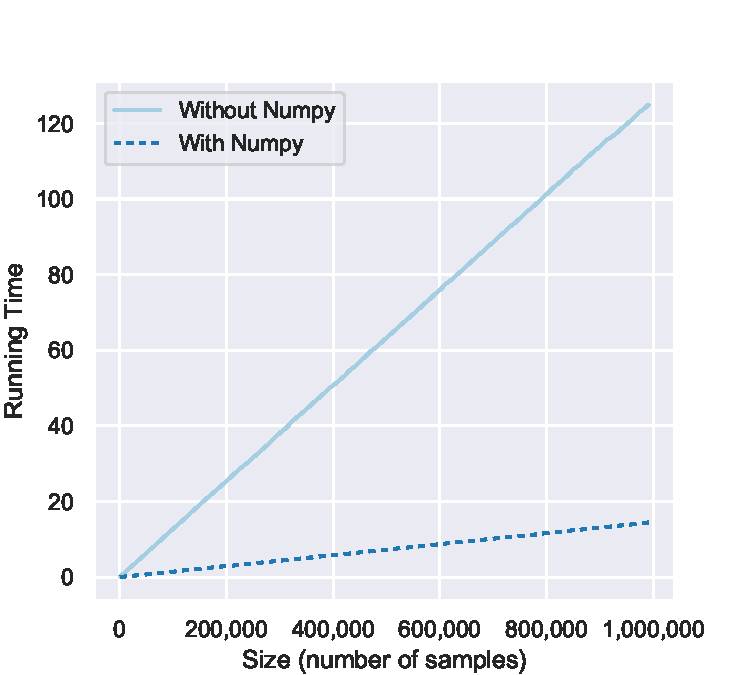
\includegraphics{serial_test.pdf}
    \end{center}
    \caption{Bootstrapping Test for Serial Functions: Performance depending on number of samples}\label{fig:SerialTest}
\end{figure}

\subsection{Parallel Algorithms}\label{subsec:parallel-algorithms}

According to \cite{STCR} "parallel processing 'languages' provide ways of managing the work performed by different
processors in a multi-processor environment." Furthermore, these authors say that by using parallel computing one should be able
to divide the problem into smaller ones and then use the different available processors to solve the entire problem. We
can interpret from these authors that in order to use parallel computing, the problem has to be divided into smaller parts.
As seen in Algorithm \ref{alg:AB}, there are 2 main loops that could work as one loop and independently between each of
its steps. Consequently, we could be able to divide the process into smaller problems and then join them to get the
results (See Algorithm \ref{alg:ABPar} line \ref{subproblem-loop}).

\medskip

\begin{algorithm}[H]
    \KwData{A sample of a random variable $X$}
    \KwResult{A standard error and confidence interval}
    \tcc{Sampling phase and Estimation phase}
    \For{\forcond}{\label{subproblem-loop}
        \tcp{Subproblem $b$}
        select $X_{1, b}^{*}, \dots, X_{n,b}^{*}$ elements of the original data using replacement\;
        estimate $T_{n,b}^{*}$ for the $b$-th sample\;}
    \tcc{Results phase}
    estimate the square root of the variance of the statistics and the confidence interval
\caption{Parallel Bootstrapping}\label{alg:ABPar}
\end{algorithm}

\medskip

To implement the parallel computing version of the Serial Bootstrapping algorithms, we are going to use the \texttt{multiprocessing}
library, which allows the possibility of creating a \texttt{Pool} of "workers" to divide the problem and then join the
results to generate the final solution. In terms of the algorithm, the \texttt{for loop}, in line \ref{subproblem-loop} of
Algorithm \ref{alg:ABPar} is going to be replaced by a \texttt{Pool} object that will implement the function a determined
number of times ($B$) to obtain the underlying empirical distribution of the statistic. Since we have two options for the
sampling phase, i.e. with \texttt{numpy} and without it, we are going to test the performance of the functions implementing
both cases under parallel computing and compare the results, and then we will analyze the results between serial and parallel
computing.

\medskip

\begin{algorithm}[H]
   \KwData{A sample of a random variable $X$}
    \KwResult{A standard error and confidence interval}
    \tcc{Sampling phase and Estimation phase}
    \MP{with \texttt{mp.Pool(workers) as pool}}{\label{subproblem-loop-python}
        \tcp{Since there are $B$ sub-problems, the \texttt{multiprocessing Pool} object will divide the implementation
             into the number of \texttt{workers} in equal chunk sizes}
        select $X_{1, b}^{*}, \dots, X_{n,b}^{*}$ elements of the original data using replacement\;
        estimate $T_{n,b}^{*}$ for the $b$-th sample\;}
    \tcc{Results phase}
    estimate the square root of the variance of the statistics and the confidence interval
\caption{Parallel Bootstrapping Example with \texttt{multiprocessing module}}\label{alg:ABPar2}
\end{algorithm}

\medskip

It is important to mention at this point that the implementation of the function under the \texttt{multiprocessing} module
of Python is based on the repetition of a function among an iterable object. Since we are repeating the same process independently
i.e. sampling and estimating, over the same iterable objects, i.e. the arguments\footnotemark, a memory problem may appear. If the original
data is too large and we want to generate a significant amount of bootstrapping samples from it, then a list of arguments
would be a vector with a repeated copy of the data vector $B$ times. To avoid this problem we created a shared object using
the \texttt{Array} object of the \texttt{multiprocessing} module where we stored the original data array. Therefore, no
copy of the original data should get generated at each repetition.

\footnotetext{Please refer to the code to understand the meaning of the use of arguments as iterable.}

\medskip

\begin{pycode}
from pylab import *
rc('font', family='serif')
rc('font', size=8.0)
rc('legend', fontsize=8.0)
rc('font', weight='normal')
import numpy as np
import pandas as pd
import matplotlib.ticker as ticker
from scipy.stats import norm
import seaborn as sns
data = pd.read_pickle('data/NoNPvsNPv2.pkl')
data_wo = data.loc[:, ['Parallel', 'ParallelNP']]
data_wo = data_wo.rename(columns={"Parallel": "Without Numpy", "ParallelNP": "With Numpy"})
clf()
figure(figsize=(5, 4.5))
sns.set(style='darkgrid', palette='Paired')
p = sns.lineplot(data=data_wo, dashes=[(None, None), (2, 2)])
p.xaxis.set_major_formatter(ticker.FuncFormatter(lambda x, pos: '{:,.0f}'.format(x)))
p.set(xlabel = 'Size (number of samples)', ylabel = 'Running Time')
savefig('parallel_test.pdf')
\end{pycode}

\begin{figure}[H]
    \begin{center}
        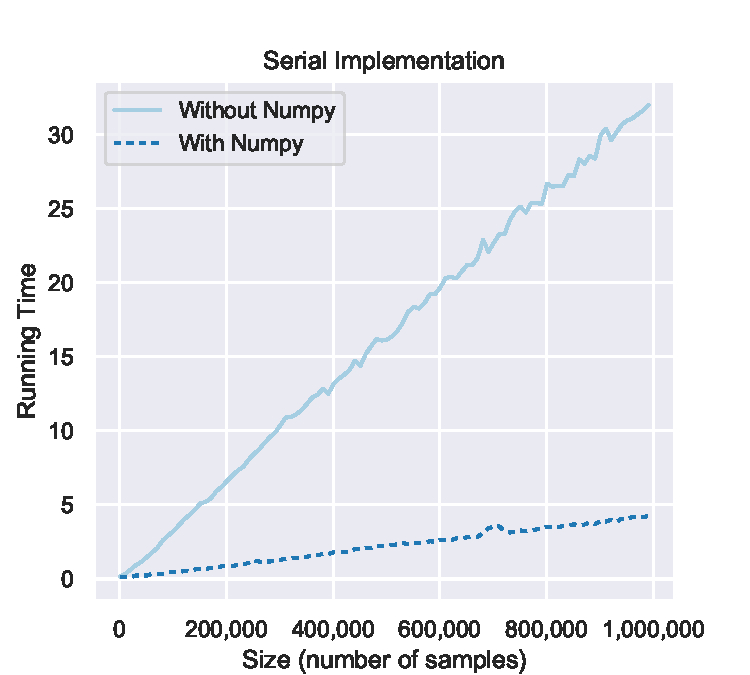
\includegraphics{parallel_test.pdf}
    \end{center}
    \caption{Bootstrapping Test for Parallel Functions: Performance depending on number of samples}\label{fig:ParallelTest}
\end{figure}

Figure \ref{fig:ParallelTest} shows the results from the implementation of the parallel version of both functions. As seen before
in the serial case, the function that uses the \texttt{numpy} package is bounded, in terms of time complexity, by the one
without it. The performance of the function with \texttt{numpy} is in average 7.26 faster than the one without it, which
is a similar result we obtained when using the serial functions. For this test, we used the total number of cores of the
computer where it was tested (i.e. 6 cores), but another important question at this point is how the performance changes
when the number of computer cores change as well. To answer the latter, we did a test of performance by using an increasing
number of cores up until the total number available in the computer (i.e. 6 cores) and leaving at $10,000$ the number of samples.
The results are presented in the Figure \ref{fig:CoresTest} and illustrate that the number of cores have a more significant
impact in the parallel version of the algorithm that does not use \texttt{numpy}, specially when it uses more than 1 core.
Contrarily, the use of \texttt{numpy} has a relevant impact for more than 2 cores, although it is not as significant
as the the case without the scientific package.

\begin{pycode}
from pylab import *
rc('font', family='serif')
rc('font', size=8.0)
rc('legend', fontsize=8.0)
rc('font', weight='normal')
import numpy as np
import pandas as pd
import matplotlib.ticker as ticker
from scipy.stats import norm
import seaborn as sns
data = pd.read_pickle('data/Cores.pkl')
data_wo = data.loc[:, ['Parallel', 'ParallelNP']]
data_wo = data_wo.rename(columns={"Parallel": "Without Numpy", "ParallelNP": "With Numpy"})
data_wo['Cores'] = data_wo.index
data_wo2 = pd.melt(data_wo, ['Cores'], var_name='Function')
clf()
figure(figsize=(5, 4.5))
sns.set(style='darkgrid', palette='Paired')
p = sns.catplot(data=data_wo2, x='Cores', y='value', hue='Function', kind='point', linestyles=["-", "--", "-", "--"],
                legend_out=False)
p.set(xlabel='Cores Used for Parallel', ylabel='Time')
savefig('cores_test.pdf')
\end{pycode}

\begin{figure}[H]
    \begin{center}
        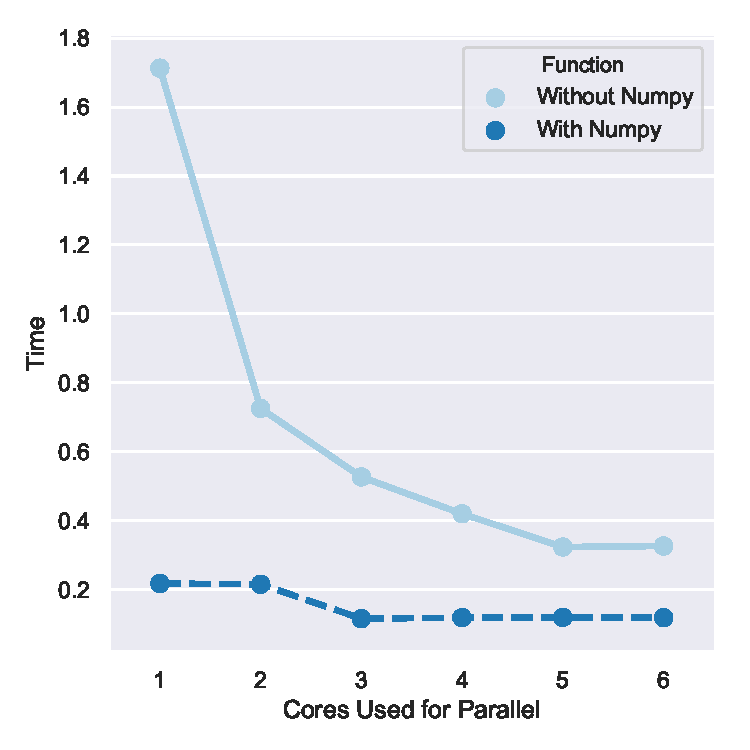
\includegraphics{cores_test.pdf}
    \end{center}
    \caption{Bootstrapping Test for Parallel Functions: Performance depending on number of Cores and executing $10,000$ samples}\label{fig:CoresTest}
\end{figure}

\subsection{Comparing Serial to Parallel Functions}

After observing the results of using the \texttt{numpy} package on both serial and parallel functions, we are going to
analyze the performance between the serial and the parallel version of each function. In this case, we should expect an
improvement in both cases, from serial to parallel, and faster performance for the \texttt{numpy} version of each function.

\begin{pycode}
from pylab import *
rc('font', family='serif')
rc('font', size=8.0)
rc('legend', fontsize=8.0)
rc('font', weight='normal')
import numpy as np
import pandas as pd
import matplotlib.ticker as ticker
from scipy.stats import norm
import seaborn as sns
data = pd.read_pickle('data/NoNPvsNPv2.pkl')
clf()
figure(figsize=(5, 4.5))
sns.set(style='darkgrid', palette='Paired')
p = sns.lineplot(data=data, dashes=[(None, None), (2, 2), (None, None), (2, 2)])
p.set(xlabel = 'Size (number of samples)', ylabel = 'Running Time')
p.xaxis.set_major_formatter(ticker.FuncFormatter(lambda x, pos: '{:,.0f}'.format(x)))
p.legend(labels=['Serial', 'Parallel', 'Serial with Numpy', 'Parallel with Numpy'])
savefig('serialvsparallel_test.pdf')
\end{pycode}

\begin{figure}[H]
    \begin{center}
        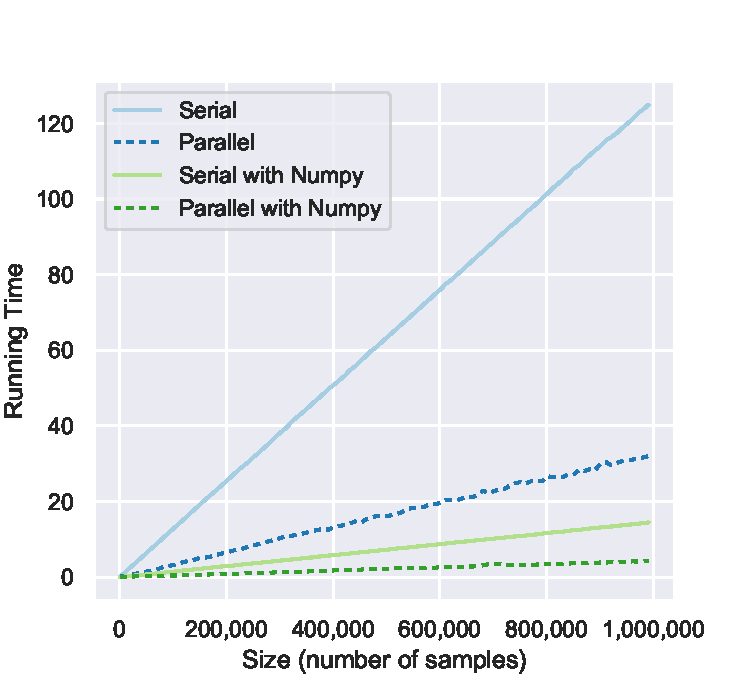
\includegraphics{serialvsparallel_test.pdf}
    \end{center}
    \caption{Bootstrapping Test for Serial and Parallel Functions: Performance depending on number of samples}\label{fig:SerialVSParallelTest}
\end{figure}

Figure \ref{fig:SerialVSParallelTest} includes all the previous results, and, as expected, the parallel versions have a
faster performance than the serial ones. Nonetheless, it is noteworthy the fact that the serial version with \texttt{numpy}
has a better performance (2.29 times) than the parallel version without it. This suggests that the \texttt{numpy} package
improves the performance of the algorithm even when it is not parallelize. Additionally, when comparing the serial version without
\texttt{numpy} and the parallel with it, the performance of the algorithm is, in average, 28.4 faster. Although the results
seem consistent along the number of samples, we analyze the performance for smaller number of samples. Figure \ref{fig:SerialVSParallelSmallTest}
shows that the serial versions of the function seems to have better performance when the size of samples is lower than
$10,000$. This results could be related with the series of steps that the \texttt{multiprocessing} module has to execute
to create the \texttt{Pool} object and the tasks related to it. This overhead can be seen as a cost for the algorithm when
a low level of samples are generated.

\begin{pycode}
from pylab import *
rc('font', family='serif')
rc('font', size=8.0)
rc('legend', fontsize=8.0)
rc('font', weight='normal')
import numpy as np
import pandas as pd
import matplotlib.ticker as ticker
from scipy.stats import norm
import seaborn as sns
data = pd.read_pickle('data/NoNPvsNP_small.pkl')
clf()
figure(figsize=(5, 4.5))
sns.set(style='darkgrid', palette='Paired')
p = sns.lineplot(data=data, dashes=[(None, None), (2, 2), (None, None), (2, 2)])
p.set(xlabel = 'Size (number of samples)', ylabel = 'Running Time')
p.xaxis.set_major_formatter(ticker.FuncFormatter(lambda x, pos: '{:,.0f}'.format(x)))
p.legend(labels=['Serial', 'Parallel', 'Serial with Numpy', 'Parallel with Numpy'])
savefig('serialvsparallel_small_test.pdf')
\end{pycode}

\begin{figure}[H]
    \begin{center}
        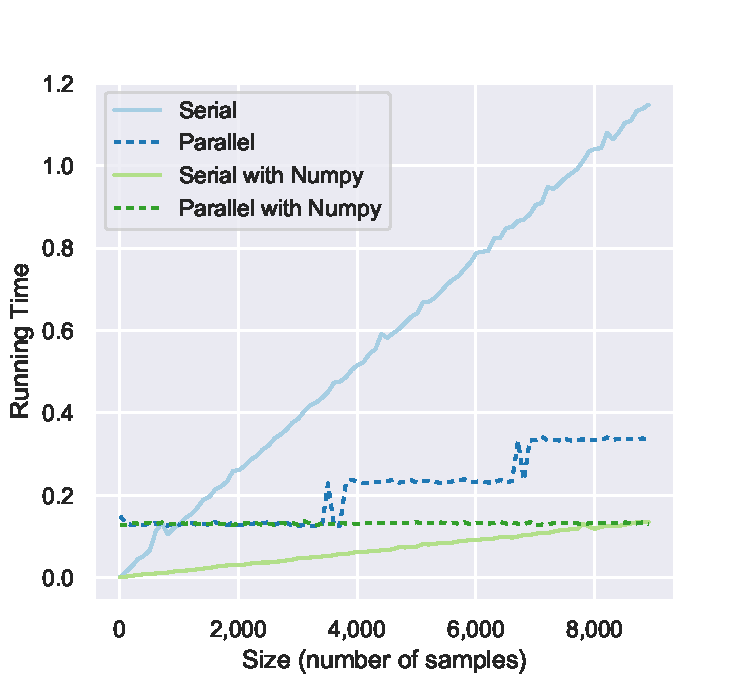
\includegraphics{serialvsparallel_small_test.pdf}
    \end{center}
    \caption{Bootstrapping Test for Serial and Parallel Functions: Performance depending on number of samples between $10$ and $5,000$}\label{fig:SerialVSParallelSmallTest}
\end{figure}

\subsection{Task Division: Separating Sampling and Estimation}\label{subsec:task-divition:-separating-sampling-and-estimation}

The previous section illustrates that the parallel versions of the bootstrapping algorithm proposed in the the present study
has have better performance, specially when special scientific packages are used to optimize it. However, when the number
of samples was lower than $10,000$ the serial version had a better performance, demonstrating that parallel computing has
limitations. These limitations seems to be related with a time overhead needed to develop the framework
for the parallel implementation. To further analyze this limitations we divided the
sampling phase from the estimation phase and construct a function for each of these phases, a serial and a parallel version.
For the parallel version we used two types of implementations, one with shared memory and one without shared memory.

\begin{pycode}
from pylab import *
rc('font', family='serif')
rc('font', size=8.0)
rc('legend', fontsize=8.0)
rc('font', weight='normal')
import numpy as np
import pandas as pd
import matplotlib.ticker as ticker
from scipy.stats import norm
import seaborn as sns
data = pd.read_pickle('data/DivParv2.pkl')
clf()
figure(figsize=(5, 4.5))
sns.set(style='darkgrid', palette="GnBu_d")
p = sns.lineplot(data=data.iloc[:, 0:3], dashes=[(None, None), (2, 2), (3, 3)])
p.set(xlabel = 'Size (number of samples)', ylabel = 'Running Time')
p.xaxis.set_major_formatter(ticker.FuncFormatter(lambda x, pos: '{:,.0f}'.format(x)))
p.legend(labels=['Sampling Serial', 'Sampling Parallel', 'Sampling Parallel Shared'])
savefig('serialvsparallel_sampling.pdf')
\end{pycode}

\begin{figure}[H]
    \begin{center}
        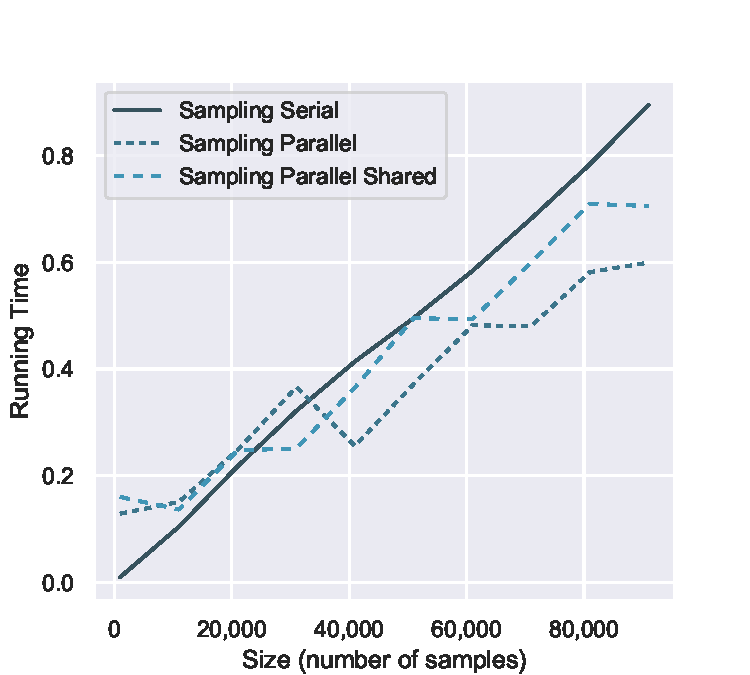
\includegraphics{serialvsparallel_sampling.pdf}
    \end{center}
    \caption{Sampling Test for Serial and Parallel Functions: Performance depending on number of samples}\label{fig:SamplingTest}
\end{figure}

The test applied to the sampling phase is presented on Figure \ref{fig:SamplingTest}, where one can see that the serial
version performs better when the levels of samples is still low. However, when the samples reaches a level near $30,000$
the parallel version of the sampling function overpasses the performance of the serial. Additionally, we can observe
that the difference between using a shared memory and not using it is not significant, but suggests a possible overhead
due to the use of a framework to share the object among the workers.

\begin{pycode}
from pylab import *
rc('font', family='serif')
rc('font', size=8.0)
rc('legend', fontsize=8.0)
rc('font', weight='normal')
import numpy as np
import pandas as pd
import matplotlib.ticker as ticker
from scipy.stats import norm
import seaborn as sns
data = pd.read_pickle('data/DivParv2.pkl')
clf()
figure(figsize=(5, 4.5))
sns.set(style='darkgrid', palette="GnBu_d")
p = sns.lineplot(data=data.iloc[:, 3:], dashes=[(None, None), (2, 2), (3, 3)])
p.set(xlabel = 'Size (number of samples)', ylabel = 'Running Time')
p.xaxis.set_major_formatter(ticker.FuncFormatter(lambda x, pos: '{:,.0f}'.format(x)))
p.legend(labels=['Statistic Serial', 'Statistic Parallel', 'Statistic Parallel Shared'])
savefig('serialvsparallel_statistic.pdf')
\end{pycode}

\begin{figure}[H]
    \begin{center}
        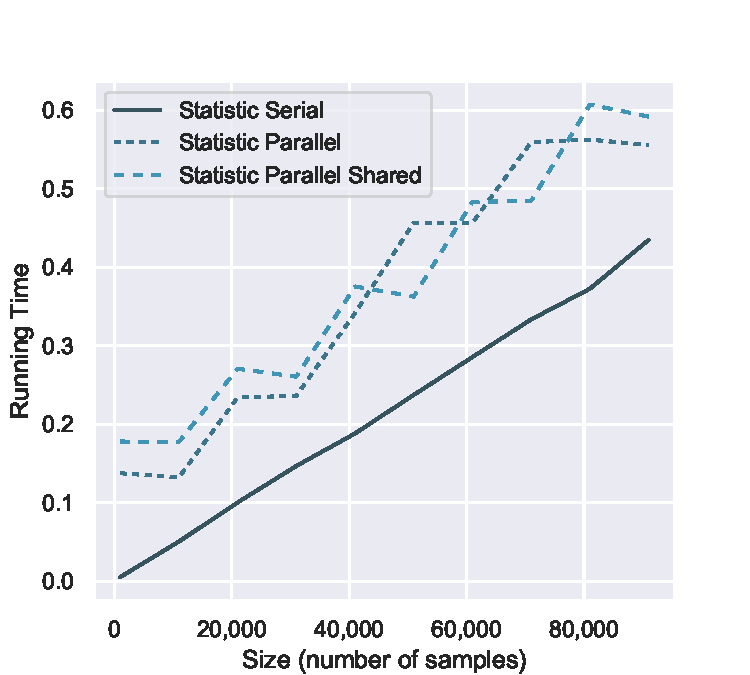
\includegraphics{serialvsparallel_statistic.pdf}
    \end{center}
    \caption{Statistic Test for Serial and Parallel Functions: Performance depending on number of samples}\label{fig:StatisticTest}
\end{figure}

The other phase to be tested is the estimation, which essentially is applying the statistic's function over each sample.
As said before, the time complexity at this phase is linear $O(n)$, although it depends on the type of statistic we are
trying to estimate. The time complexity of the function applied could affect the performance of the algorithm, so the
results presented at this point are related to applying a simple statistic as the mean. Figure \ref{fig:StatisticTest}
contains the results of the test to measure the performance among different sample sizes. The serial version seems to
run faster even for a larger number of samples up until reaching the maximum of the test (i.e. $100,000$)\footnotemark. We
believe that this performance is due to the fact that the overhead timing of the parallel implementation is too long for
a simple task as computing a "simple" function to $B$ samples. Therefore, we believe that parallel version of the estimation
phase is useful only when the function to estimate the statistic is complex enough to take a significant amount of time.

\footnotetext{We tried to estimate the same test parameters as the previous tests, but the running time exceeded 36 hours.
              Therefore, we decided to maintain the results presented at the graph. Nonetheless, is important
              to mention that the conclusions may vary for larger number of samples.}

\section{Conclusions: Benefits and Costs of using parallel computing for Bootstrapping}

The main algorithm to estimate the bootstrapping's standard errors and the confidence intervals showed a result aligned with
the theory, as presented in Section \ref{subsec:basic-algorithm}. Furthermore, the serial and parallel versions showed the same
results as the initial algorithm. In regard to the performance the first results showed that the parallel version took less
time to accomplish the tasks under certain conditions.

\medskip

First, it is important to understand that the sampling phase had the highest time complexity of the phases of the algorithm, since it has to
perform a series of \texttt{for loops}\footnotemark to construct each sample. Therefore, the general algorithm should have
benefited from parallel computing at the sampling phase. Contrarily, the estimation phase, in the specific case of the mean,
just performed a single \texttt{loop} to apply the function $B$ times. Nonetheless, this result was conditioned on the
number of samples (i.e. $B$), since from 0 to an specific point (nearly $1,000$ samples for the serial without \texttt{numpy}
and just over $8,000$ samples for the serial with \texttt{numpy}) the serial version was faster than the parallel one. As
said before, we believe that the main reason for this behavior is the parallel overhead, which is a cost up until the
points mentioned, after these points, the parallel functions have the benefit of improve the performance.

\medskip

Secondly, the division of the task to simpler tasks showed that as the process is simpler the parallel overhead remains a cost
for longer input sizes. Figure \ref{fig:StatisticTest} exemplified this statement, since the serial version of the estimation
of the statistic remained faster than the parallel one. Therefore, for simpler tasks, the parallel implementation may
possess a significant timing overhead, demonstrating that the use of parallel computing should be used with more elaborated
processes than just applying a simple function along a array.

\medskip

Finally, we consider that there a number of extensions that could be done to further analyze the impact of parallel computing
on the bootstrapping algorithm. One first extension is varying the statistic used, for example using the median or more elaborate ones;
a second extension could be implementing the divided version with larger inputs to determine if there exist a point where
the serial version is bounded by the parallel when using the mean as statistic; thirdly, one could generate samples as big
as the original data to check if the time complexity reaches a polynomial of 2nd degree; and, finally, include the estimation
of a series of statistics like the standard error and the confidence intervals (including the different types of CI's) to
observe the impact. Altough it is not a direct extension of the presentation, there is a variation of the bootstrap algorithm
that includes the poisson distribution to create a matrix with the counts of each observation in each sample, therefore reducing
the possible loops to generate random samples.



\footnotetext{The \texttt{numpy}'s code shows that the process of random generation is done in \texttt{C}, which reduces
              the time, but still seems to perform a loop to fill the array.}

\printbibliography

\section{Appendix: Code}

\subsection{Serial and Parallel functions}

\begin{Verbatim}[fontsize=\tiny]
import multiprocessing as mp
from multiprocessing.pool import ApplyResult

import numpy as np
import ctypes
from random import randint
import timeit
import matplotlib.pyplot as plt
import pandas as pd
import seaborn as sns
from typing import Callable, List

# Boostrapping without Numpy
from traitlets import List


def bootstrap(x: np.ndarray, func: Callable, samples: int = 100, sample_size: int = 0) -> list:
    """
    This function generates a determined number of samples from an initial array and apply to each the
    function of the statistic. It uses the random library to randomize the indexes for sampling.

    Parameters
    ----------
    x : np.ndarray
        Structure of data to apply the bootstrapping process
    func : function
        Function of how to apply the statistic (ex. mean, std, etc.)
    samples : int
        Number of samples to take from x
    sample_size :   int
        Size of each sample, should be between 0 and the total length of x

    Returns
    -------
    list
        A list with the result of applying the function to each sample

    Examples
    --------
    Generate a bootstrap distribution of the mean of a sample from a normal distribution(5, 1)
    >>> sample_normal = np.random.normal(5, 1, 1000)
    >>> bootstrap(sample_normal, np.mean, samples = 1000, sample_size = 100)
    """

    assert isinstance(x, np.ndarray), "Please convert the input into an numpy ndarray"

    if sample_size == 0:
        sample_size = len(x)

    def extract(y):
        rindex = [randint(0, len(x) - 1) for _ in range(sample_size)]
        return [y[i] for i in rindex]

    return [func(extract(x)) for _ in range(samples)]


# Bootstrapping with Numpy
def bootstrap_np(x: np.ndarray, func: Callable, samples: int = 1000, sample_size: int = 100) -> list:
    """
    This function generates a determined number of samples from an initial array and apply to each the
    function of the statistic. It uses Numpy to reduce the running time.

    Parameters
    ----------
    x : np.ndarray
        Structure of data to apply the bootstrapping process
    func : function
        Function of how to apply the statistic (ex. mean, std, etc.)
    samples : int
        Number of samples to take from x
    sample_size :   int
        Size of each sample, should be between 0 and the total length of x

    Returns
    -------
    list
        A list with the result of applying the function to each sample

    Examples
    --------
    Generate a bootstrap distribution of the mean of a sample from a normal distribution(5, 1)
    >>> sample_normal = np.random.normal(5, 1, 1000)
    >>> bootstrap_np(sample_normal, np.mean, samples = 1000, sample_size = 100)
    """
    return [func(np.random.choice(x, sample_size)) for _ in range(samples)]


def bootstrap_par_comp(x: np.ndarray, func: Callable, sample_size: int) -> float:
    """
    This function generates a determined number of samples from an initial array and apply to each the
    function of the statistic. It does not uses numpy to randomize the samples. This function will be used
    to define a new function which uses parallel computing. It is define outside the parallel function to
    avoid error from the multiprocessing module.

    Parameters
    ----------
    x : np.ndarray
        Structure of data to apply the bootstrapping process
    func : function
        Function of how to apply the statistic (ex. mean, std, etc.)
    sample_size :   int
        Size of each sample, should be between 0 and the total length of x

    Returns
    -------
    float
        A float as a result of the function applied to the specific samples size.

    Examples
    --------
    Generate a sample of a normal distribution and estimate the mean of it.
    >>> sample_normal = np.random.normal(5, 1, 1000)
    >>> bootstrap_par_comp(sample_normal, np.mean, sample_size = 100)
    """
    rindex = [randint(0, len(x) - 1) for _ in range(sample_size)]
    return func([x[i] for i in rindex])


# Boostrapping in parallel without Numpy
def bootstrap_par(x: np.ndarray, func: Callable, samples: int = 100, sample_size: int = 0, workers=0) -> list:
    """
    This function generates a determined number of samples from an initial array and apply to each the
    function of the statistic. It uses the multiprocessing module to create a pool of workers to divide the
    input into equal sizes (i.e. divides the list of samples). Important to notice that the structure of data
    is created as a memory shared array to avoid incurring in creating multiple copies of it.

    Parameters
    ----------
    x : np.ndarray
        Structure of data to apply the bootstrapping process
    func : function
        Function of how to apply the statistic (ex. mean, std, etc.)
    samples : int
        Number of samples to take from x
    sample_size :   int
        Size of each sample, should be between 0 and the total length of x

    Returns
    -------
    list
        A list with the result of applying the function to each sample

    Examples
    --------
    Generate a bootstrap distribution of the mean of a sample from a normal distribution(5, 1)
    >>> sample_normal = np.random.normal(5, 1, 1000)
    >>> bootstrap_par(sample_normal, np.mean, samples = 1000, sample_size = 100)
    """
    if sample_size == 0:
        sample_size = len(x)

    if workers == 0:
        workers = mp.cpu_count()

    x_ = mp.Array(ctypes.c_double, len(x))
    x_shr = np.ctypeslib.as_array(x_.get_obj())
    x_shr[:] = x

    with mp.Pool(workers) as pool:
        results = pool.starmap_async(bootstrap_par_comp,
                                     [(x_shr, func, sample_size) for _ in range(samples)]).get()

    pool.close()
    return results


def bootstrap_complete(x: np.ndarray, func: Callable, sample_size: int) -> float:
    """
    This function generates a determined number of samples using the module random of numpy from an initial array
    and apply to each the function of the statistic. The function will be used to define a new function which
    uses parallel computing. It is define outside the parallel function to avoid error from the multiprocessing
    module.

    Parameters
    ----------
    x : np.ndarray
        Structure of data to apply the bootstrapping process
    func : function
        Function of how to apply the statistic (ex. mean, std, etc.)
    sample_size :   int
        Size of each sample, should be between 0 and the total length of x

    Returns
    -------
    float
        A float as a result of the function applied to the specific samples size.

    Examples
    --------
    Generate a sample of a normal distribution and estimate the mean of it.
    >>> sample_normal = np.random.normal(5, 1, 1000)
    >>> bootstrap_complete(sample_normal, np.mean, sample_size = 100)
    """
    return func(np.random.choice(x, sample_size))


# Bootstrapping in parallel with Numpy
def bootstrap_np_par(x: np.ndarray, func: Callable, samples: int = 1000, sample_size: int = 100, workers=0):
    """
     This function generates a determined number of samples from an initial array and apply to each the
     function of the statistic. It uses the multiprocessing module to create a pool of workers to divide the
     input into equal sizes (i.e. divides the list of samples). Important to notice that the structure of data
     is created as a memory shared array to avoid incurring in creating multiple copies of it.

     Parameters
     ----------
     x : np.ndarray
         Structure of data to apply the bootstrapping process
     func : function
         Function of how to apply the statistic (ex. mean, std, etc.)
     samples : int
         Number of samples to take from x
     sample_size :   int
         Size of each sample, should be between 0 and the total length of x

     Returns
     -------
     list
         A list with the result of applying the function to each sample

     Examples
     --------
     Generate a bootstrap distribution of the mean of a sample from a normal distribution(5, 1)
     >>> sample_normal = np.random.normal(5, 1, 1000)
     >>> bootstrap_par(sample_normal, np.mean, samples = 1000, sample_size = 100)
     """
    if workers == 0:
        workers = mp.cpu_count()

    x_ = mp.Array(ctypes.c_double, len(x))
    x_shr = np.ctypeslib.as_array(x_.get_obj())
    x_shr[:] = x

    with mp.Pool(workers) as pool:
        results: List[float] = pool.starmap_async(bootstrap_complete,
                                                  [(x_shr, func, sample_size) for _ in range(samples)]).get()

    pool.close()
    return results

\end{Verbatim}


\subsection{Tests of Serial and Parallel functions}

\begin{Verbatim}[fontsize=\tiny]
###############################
#### Test-size-resample.py ####
###############################

import numpy as np
import timeit
import matplotlib.pyplot as plt
import pandas as pd
import seaborn as sns

s = '''
sample_normal = np.random.normal(5, 1, 10000)
test = parallel_bootstrap.bootstrap(sample_normal, np.mean, {}, 100)
'''

setup = '''
import numpy as np
from src import parallel_bootstrap
'''

s_np = '''
sample_normal = np.random.normal(5, 1, 10000)
test = parallel_bootstrap.bootstrap_np(sample_normal, np.mean, {}, 100)
'''

setup_np = '''
import numpy as np
from src import parallel_bootstrap
'''

s_par = '''
sample_normal = np.random.normal(5, 1, 10000)
test_p = parallel_bootstrap.bootstrap_par(sample_normal, np.mean, {}, 100)
'''

setup_par = '''
import multiprocessing as mp
import numpy as np
from src import parallel_bootstrap
'''

s_np_par = '''
sample_normal = np.random.normal(5, 1, 10000)
test_p = parallel_bootstrap.bootstrap_np_par(sample_normal, np.mean, {}, 100)
'''

setup_np_par = '''
import multiprocessing as mp
import numpy as np
from src import parallel_bootstrap
'''

instructions_s = [s.format(i) for i in range(10, 9000, 100)]
instructions_s_par = [s_par.format(i) for i in range(10, 9000, 100)]
instructions_s_np = [s_np.format(i) for i in range(10, 9000, 100)]
instructions_s_np_par = [s_np_par.format(i) for i in range(10, 9000, 100)]

serial = [timeit.Timer(stmt=ins, setup=setup).timeit(1) for ins in instructions_s]
par = [timeit.Timer(stmt=ins, setup=setup_par).timeit(1) for ins in instructions_s_par]
np_serial = [timeit.Timer(stmt=ins, setup=setup_np).timeit(1) for ins in instructions_s_np]
np_par = [timeit.Timer(stmt=ins, setup=setup_np_par).timeit(1) for ins in instructions_s_np_par]
repeats = range(10, 9000, 100)

df = pd.DataFrame(np.c_[serial, par, np_serial, np_par], index=repeats,
                  columns=['Serial', 'Parallel', 'SerialNP', 'ParallelNP'])

df.to_pickle('../data/NoNPvsNP_small.pkl')

sns.set(style='darkgrid', palette='Paired')
sns.lineplot(data=df, dashes=[(None, None), (2, 2), (None, None), (2, 2)])
plt.legend(labels=['Serial', 'Parallel', 'Serial with Numpy', 'Parallel with Numpy'])
plt.show()

##############################
#### Test-number-cores.py ####
##############################

import numpy as np
import timeit
import matplotlib.pyplot as plt
import pandas as pd
import seaborn as sns
from src import parallel_bootstrap

s_par = '''
sample_normal = np.random.normal(5, 1, 10000)
test_p = parallel_bootstrap.bootstrap_par(sample_normal, np.mean, 10000, 100, {})
'''

setup_par = '''
import multiprocessing as mp
import numpy as np
from src import parallel_bootstrap
'''

s_np_par = '''
sample_normal = np.random.normal(5, 1, 10000)
test_p = parallel_bootstrap.bootstrap_np_par(sample_normal, np.mean, 10000, 100, {})
'''

setup_np_par = '''
import multiprocessing as mp
import numpy as np
from src import parallel_bootstrap
'''


instructions_s_par = [s_par.format(i) for i in range(1, 7, 1)]
instructions_s_np_par = [s_np_par.format(i) for i in range(1, 7, 1)]


par = [timeit.Timer(stmt=ins, setup=setup_par).timeit(1) for ins in instructions_s_par]
np_par = [timeit.Timer(stmt=ins, setup=setup_np_par).timeit(1) for ins in instructions_s_np_par]
cores = range(1, 7, 1)

df = pd.DataFrame(np.c_[par, np_par], index=cores,
                  columns=['Parallel', 'ParallelNP'])

df.to_pickle('../data/Cores.pkl')

df['Cores'] = df.index
df2 = pd.melt(df, ['Cores'], var_name='Function')
sns.set(style='darkgrid', palette='Paired')
p = sns.catplot(data=df2, x='Cores', y='value', hue='variable', kind='point', linestyles=["-", "--", "-", "--"],
                legend_out=False)
p.set(xlabel='Cores Used for Parallel', ylabel='Time')
p.fig.text(2.2, 0.9, '*Serial presented for comparison.')
plt.show()

\end{Verbatim}

\subsection{Divided version of Serial and Parallel functions}

\begin{Verbatim}[fontsize=\tiny]
import numpy as np
import multiprocessing as mp
import ctypes
from typing import Callable


def sampling(x, samples=1000, sample_size=100):
    """
    This function generates a determined number of samples from an initial array.
    It uses the numpy library to randomly sample from the initial array.

    Parameters
    ----------
    x : np.ndarray
        The array of data to which the sampling process is applied
    samples : int
        Number of samples to take from x
    sample_size :   int
        Size of each sample, should be between 0 and the total length of x

    Returns
    -------
    np.ndarray
        An array of all samples taken from x, where each sample is an array
        of size sample_size.

    Examples
    --------
    Given an array of data taken from a normal distribution(5, 1), take 1000 samples
    of size 100 from the data.
    >>> sample_normal = np.random.normal(5, 1, 1000)
    >>> sampling(sample_normal, samples = 1000, sample_size = 100)
    """
    return np.array([np.random.choice(x, sample_size) for _ in range(samples)])


def sampling_par(x, samples=1000, sample_size=100):
    """
    This function generates a determined number of samples from an initial array.
    It uses the numpy library to randomly sample from the initial array. Using the
    multiprocessing package it parallelises the process by creating a
    pool of workers and dividing up the sampling tasks between them. The number of
    workers is the same as the number of CPUs in the computer.

    Parameters
    ----------
    x : np.ndarray
        The array of data to which the sampling process is applied
    samples : int
        Number of samples to take from x
    sample_size :   int
        Size of each sample, should be between 0 and the total length of x

    Returns
    -------
    np.ndarray
        An array of all samples taken from x, where each sample is an array
        of size sample_size.

    Examples
    --------
    Given an array of data taken from a normal distribution(5, 1), take 1000 samples
    of size 100 from the data.
    >>> sample_normal = np.random.normal(5, 1, 1000)
    >>> sampling_par(sample_normal, samples = 1000, sample_size = 100)
    """
    with mp.Pool(processes=mp.cpu_count()) as pool:
        results = pool.starmap_async(np.random.choice, [(x, sample_size) for _ in range(samples)]).get()
    pool.close()
    return results


def sampling_par_shared(x, samples=1000, sample_size=100):
    """
    This function generates a determined number of samples from an initial array.
    It uses the numpy library to randomly sample from the initial array. Using the
    multiprocessing package it parallelises the process by creating a
    pool of workers and dividing up the sampling tasks between them. Before parallelisation,
    the initial numpy array is turned into a memory shared array, meaning that the
    array can be shared by the workers and avoids creating multiple copies of it.
    The number of workers is the same as the number of CPUs in the computer.

    Parameters
    ----------
    x : np.ndarray
        The array of data to which the sampling process is applied
    samples : int
        Number of samples to take from x
    sample_size :   int
        Size of each sample, should be between 0 and the total length of x

    Returns
    -------
    np.ndarray
        An array of all samples taken from x, where each sample is an array
        of size sample_size.

    Examples
    --------
    Given an array of data taken from a normal distribution(5, 1), take 1000 samples
    of size 100 from the data.
    >>> sample_normal = np.random.normal(5, 1, 1000)
    >>> sampling_par_shared(sample_normal, samples = 1000, sample_size = 100)
    """
    x_ = mp.Array(ctypes.c_double, len(x))
    x_shr = np.ctypeslib.as_array(x_.get_obj())
    x_shr[:] = x

    with mp.Pool(mp.cpu_count()) as pool:
        results = pool.starmap_async(np.random.choice, [(x, sample_size) for _ in range(samples)]).get()
    pool.close()
    return results


def statistic(x, func):
    """
    This function applies a determined function to each sample in the input array of samples.

    Parameters
    ----------
    x : np.ndarray
        The array of samples, where each sample is an array, for which
        the statistic function is applied to each sample
    func : function
        The statistical function to be applied to each sample in x

    Returns
    -------
    np.ndarray
        An array of outputs from the function applied to each sample

    Examples
    --------
    Given an array of data taken from a normal distribution(5, 1), take 1000 samples
    of size 100 from the data. Given this array of samples, get the mean for each sample.
    >>> sample_normal = np.random.normal(5, 1, 1000)
    >>> samples = sampling(sample_normal, samples = 1000, sample_size = 100)
    >>> sample_means = statistic(samples, func = np.mean)
    """
    return np.array([func(z) for z in x])


def statistic_par(x, func):
    """
    This function applies a determined function to each sample in the input array of samples.
    Using the multiprocessing package it parallelises the process by creating a pool of
    workers and dividing up the tasks between them. The number of workers is the same as
    the number of CPUs in the computer.

    Parameters
    ----------
    x : np.ndarray
        The array of samples, where each sample is an array, for which
        the statistic function is applied to each sample
    func : function
        The statistical function to be applied to each sample in x

    Returns
    -------
    np.ndarray
        An array of outputs from the function applied to each sample

    Examples
    --------
    Given an array of data taken from a normal distribution(5, 1), take 1000 samples
    of size 100 from the data. Given this array of samples, get the mean for each sample.
    >>> sample_normal = np.random.normal(5, 1, 1000)
    >>> samples = sampling(sample_normal, samples = 1000, sample_size = 100)
    >>> sample_means = statistic(samples, func = np.mean)
    """
    with mp.Pool(processes=mp.cpu_count()) as pool:
        results = pool.map_async(func, x).get()
    pool.close()
    return results


def statistic_par_shared(x: np.ndarray, func: Callable):
    """
    This function applies a determined function to each sample in the input array of samples.
    Using the multiprocessing package it parallelises the process by creating a pool of
    workers and dividing up the tasks between them. Before parallelisation, the initial
    numpy array is turned into a memory shared array, meaning that the array can be
    shared by the workers and avoids creating multiple copies of it. The number of workers
    is the same as the number of CPUs in the computer.

    Parameters
    ----------
    x : np.ndarray
        The array of samples, where each sample is an array, for which
        the statistic function is applied to each sample
    func : function
        The statistical function to be applied to each sample in x

    Returns
    -------
    np.ndarray
        An array of outputs from the function applied to each sample

    Examples
    --------
    Given an array of data taken from a normal distribution(5, 1), take 1000 samples
    of size 100 from the data. Given this array of samples, get the mean for each sample.
    >>> sample_normal = np.random.normal(5, 1, 1000)
    >>> samples = sampling(sample_normal, samples = 1000, sample_size = 100)
    >>> sample_means = statistic(samples, func = np.mean)
    """
    x_ = [mp.Array(ctypes.c_double, len(x)) for _ in range(x.shape[1])]
    x_shr = [np.ctypeslib.as_array(z.get_obj()) for z in x_]
    x_shr[:] = x

    with mp.Pool(mp.cpu_count()) as pool:
        results = pool.map_async(func, x_shr).get()

    pool.close()
    return results
\end{Verbatim}

\subsection{Test for the divided version of Serial and Parallel functions}

\begin{Verbatim}[fontsize=\tiny]
import numpy as np
import timeit
import matplotlib.pyplot as plt
import pandas as pd
import seaborn as sns

setup_sample = '''
import numpy as np
import multiprocessing as mp
from src import parallel_bootstrap_divided
sample_normal = np.random.normal(5, 1, 1000)
'''
setup_statistic = '''
import multiprocessing as mp
import numpy as np
from src import parallel_bootstrap_divided
sample_normal = np.random.normal(5, 1, 1000)
all_samples = [sampling(sample_normal, i, 100) for i in range(1000, 100000, 10000)]
'''

s = '''
parallel_bootstrap_divided.sampling(sample_normal, samples={}, sample_size=100)
'''
s_p = '''
parallel_bootstrap_divided.sampling_par(sample_normal, samples={}, sample_size=100)
'''
s_ps = '''
parallel_bootstrap_divided.sampling_par_shared(sample_normal, samples={}, sample_size=100)
'''
st = '''
parallel_bootstrap_divided.statistic(all_samples[{}], np.mean)
'''
st_p = '''
parallel_bootstrap_divided.statistic_par(all_samples[{}], np.mean)
'''
st_ps = '''
parallel_bootstrap_divided.statistic_par_shared(all_samples[{}], np.mean)
'''
ins_sample = [s.format(i) for i in range(1000, 100000, 10000)]
ins_sample_p = [s_p.format(i) for i in range(1000, 100000, 10000)]
ins_sample_ps = [s_ps.format(i) for i in range(1000, 100000, 10000)]
ins_stat = [st.format(i) for i in range(10)]
ins_stat_p = [st_p.format(i) for i in range(10)]
ins_stat_ps = [st_ps.format(i) for i in range(10)]

sample = [timeit.Timer(stmt=ins, setup=setup_sample).timeit(1) for ins in ins_sample]
sample_p = [timeit.Timer(stmt=ins, setup=setup_sample).timeit(1) for ins in ins_sample_p]
sample_ps = [timeit.Timer(stmt=ins, setup=setup_sample).timeit(1) for ins in ins_sample_ps]
stat = [timeit.Timer(stmt=ins, setup=setup_statistic).timeit(1) for ins in ins_stat]
stat_p = [timeit.Timer(stmt=ins, setup=setup_statistic).timeit(1) for ins in ins_stat_p]
stat_ps = [timeit.Timer(stmt=ins, setup=setup_statistic).timeit(1) for ins in ins_stat_ps]

repeats = range(1000, 100000, 10000)

df = pd.DataFrame(np.c_[sample, sample_p, sample_ps, stat, stat_p, stat_ps],
                    index=repeats, columns=['Sampling', 'SamplingP', 'SamplingPS',
                                            'Statistic', 'StatisticP', 'StatisticPS'])

df.to_pickle('../data/DivParv2.pkl')

sns.set(style='darkgrid', palette='Paired')
sns.lineplot(data=df)
plt.legend(labels=['Sampling', 'SamplingP', 'SamplingPS',
                       'Statistic', 'StatisticP', 'StatisticPS'])
plt.show()

\end{Verbatim}
\end{document}